\section*{Лабораторная работа}
\textbf{Содержание проекта:} Команда разработчиков из \textbf{16 человек} занимается созданием карты города на основе собственного модуля отображения. Проект должен быть завершен в течение \textbf{6 месяцев}. Бюджет проекта: 50 000 рублей.

На рисунке \ref{p0} показаны используемые ресурсы:
\begin{figure}[!h]
	\centering
	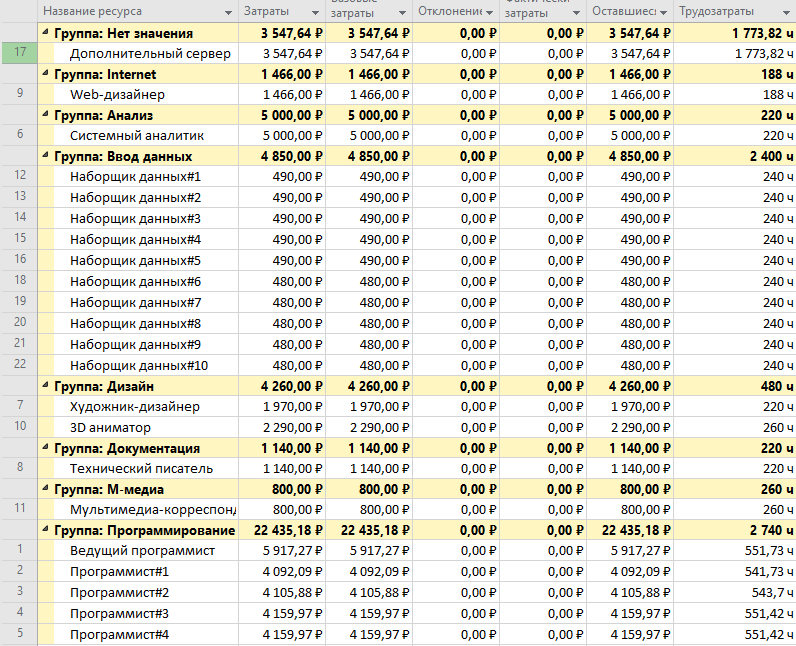
\includegraphics[width=1\linewidth]{inc/img/0.png}
	\caption{Используемые ресурсы}
	\label{p0}
\end{figure}

\newpage
\subsection*{Задание №1: Работа с таблицей освоенного объема}
После выполнение лабораторной работы №4 проект имеет следующие характеристики:

\noindent Затраты: 46 700,92 руб.

\noindent Длительность: 20,85 недель

\noindent Окончание: 01.08.23

На рисунке \ref{p1} изображена таблица освоенного объема:
\begin{figure}[!h]
	\centering
	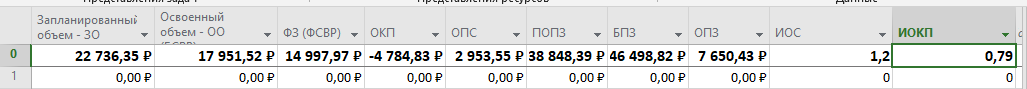
\includegraphics[width=1\linewidth]{inc/img/1.png}
	\caption{Таблица освоенного объема}
	\label{p1}
\end{figure}

По данному рисунку можно сделать следующие выводы, о показателях проекта:

\noindent ОКП < 0 => проект запаздывает

\noindent ОПС > 0 => проект находится в пределах сметы

\noindent ОПЗ > 0 => нет перерасхода средств

\newpage
\subsection*{Задание №2: Работа с отчетами проекта}
На рисунке \ref{p8} представлен отчет о бюджетной стоимости:
\begin{figure}[!h]
	\centering
	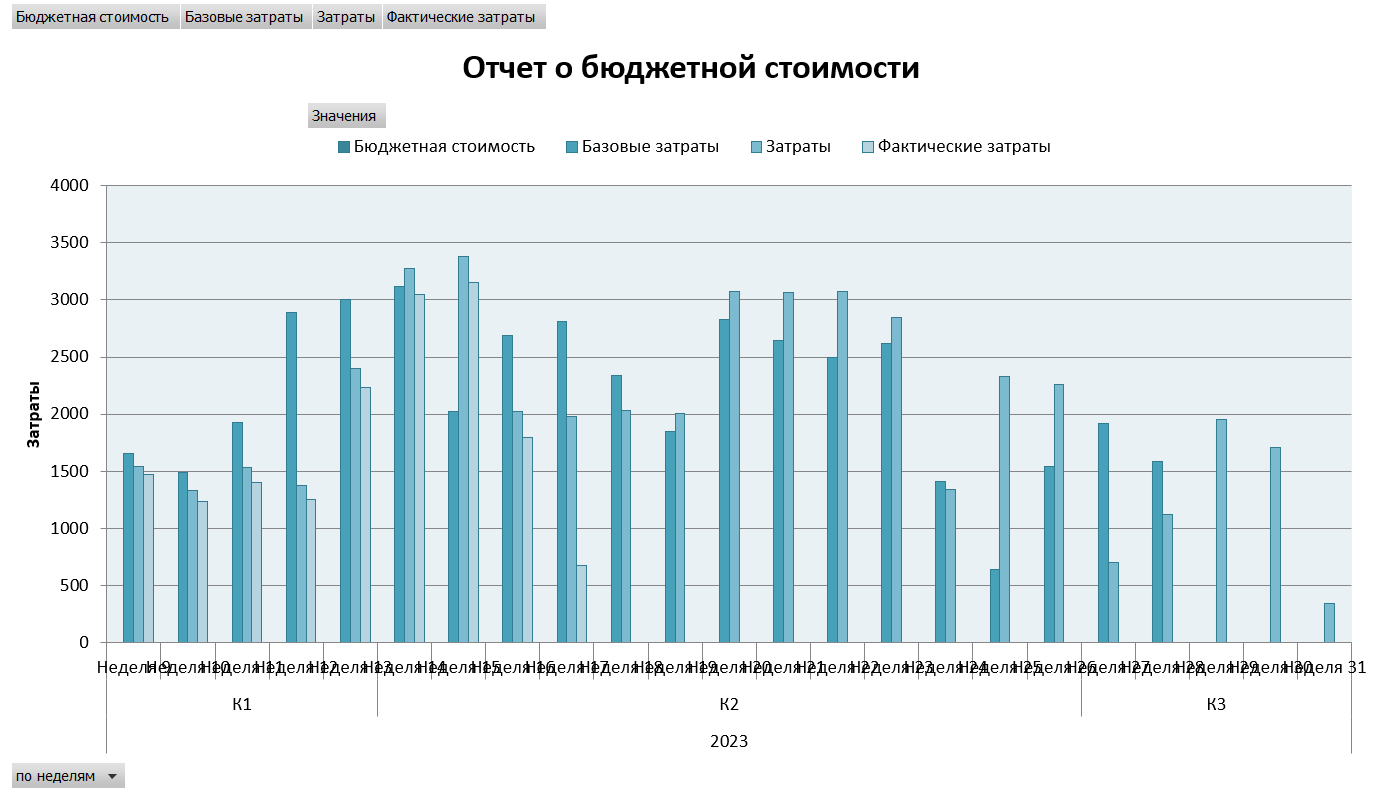
\includegraphics[width=1\linewidth]{inc/img/8.png}
	\caption{Отчет о бюджетной стоимости}
	\label{p8}
\end{figure}

По гистограмме можно сделать вывод, что наибольшая потребность в финансировании возникает на 14ой и 15ой неделях.


На рисунках \ref{p4}-\ref{p5} можно увидеть состояния затрат для задач верхнего уровня:
\begin{figure}[!h]
	\centering
	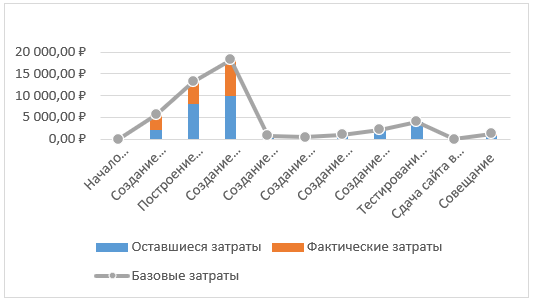
\includegraphics[width=0.7\linewidth]{inc/img/4.png}
	\caption{Состояние затрат для всех задач верхнего уровня}
	\label{p4}
\end{figure}

\newpage
\begin{figure}[!h]
	\centering
	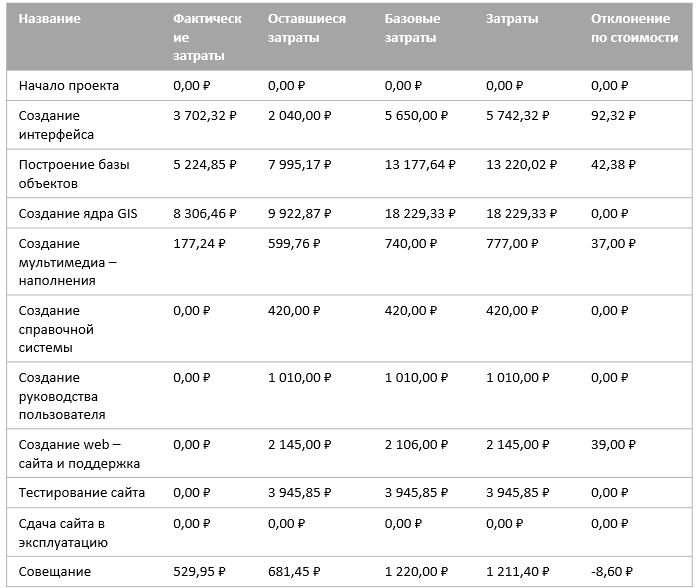
\includegraphics[width=0.7\linewidth]{inc/img/5.png}
	\caption{Состояние затрат для задач верхнего уровня}
	\label{p5}
\end{figure}

Судя по графику, можно сделать вывод, что наибольшая потребность в деньгах приходится на первую половину проекта, а именно на задачи "Создание ядра GIS" и "Построение базы объектов".

%\newpage
На рисунках \ref{p2}-\ref{p3} можно увидеть какие задачи превышают бюджетную стоимость:
\begin{figure}[!h]
	\centering
	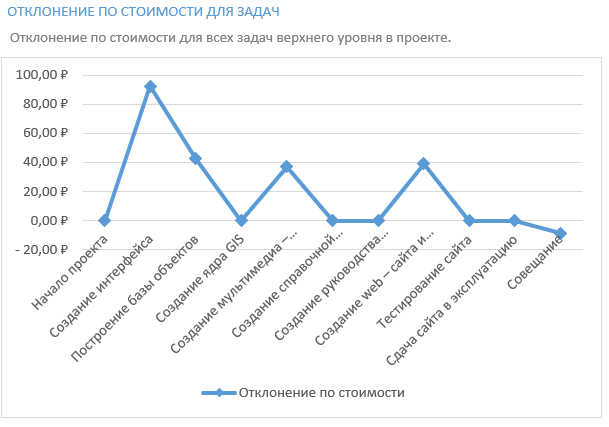
\includegraphics[width=0.7\linewidth]{inc/img/2.png}
	\caption{График превышений затрат по задачам}
	\label{p2}
\end{figure}

\newpage
\begin{figure}[!h]
	\centering
	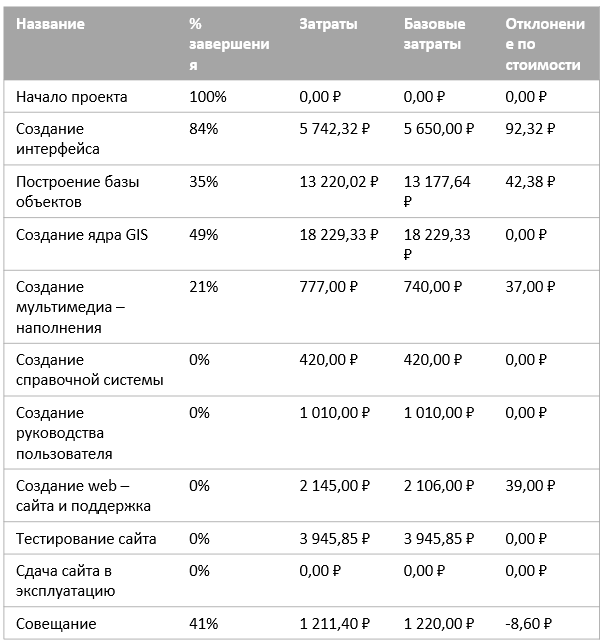
\includegraphics[width=0.7\linewidth]{inc/img/3.png}
	\caption{Таблица превышений затрат по задачам}
	\label{p3}
\end{figure}


\newpage
\subsection*{Задание №3: Анализ вариантов декомпозиции работ в проекте}
Декомпозиция до (рис. \ref{p6}):
\begin{figure}[!h]
	\centering
	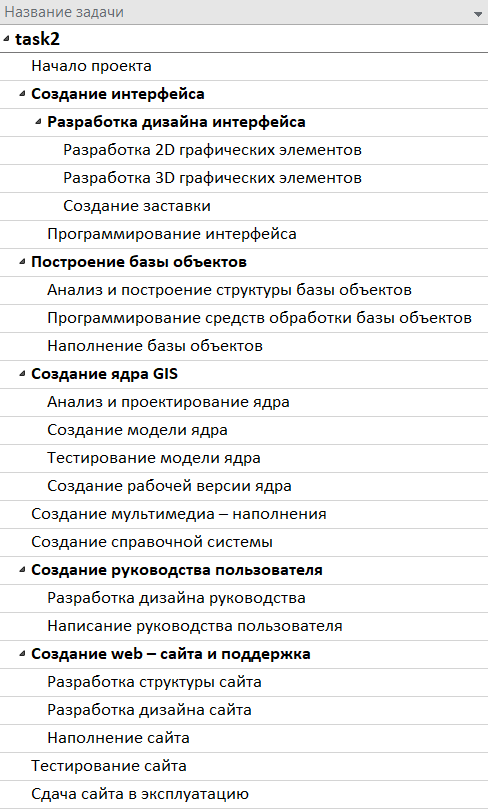
\includegraphics[width=0.7\linewidth]{inc/img/6.png}
	\caption{Декомпозиция до}
	\label{p6}
\end{figure}

\newpage
Декомпозиция после (рис. \ref{p7}):
\begin{figure}[!h]
	\centering
	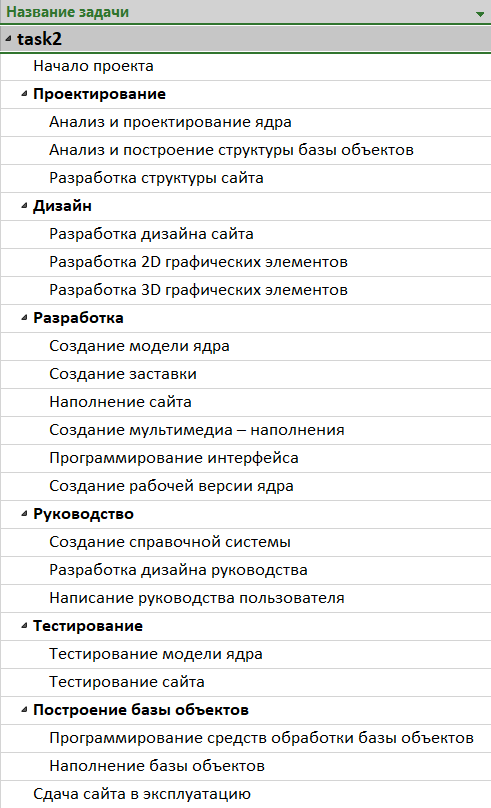
\includegraphics[width=0.7\linewidth]{inc/img/7.png}
	\caption{Декомпозиция после}
	\label{p7}
\end{figure}

В результате дата завершения проекта не изменилась (15.09.23), а затраты немного уменьшились с 48 046 руб. до 47 374 руб. т.к. аренда сервер большая не используется для задачи "Анализ и построение структуры базы объектов".

\section*{Выводы}
По таблице освоенного объема был сделан вывод, что проект запаздывает, но все еще находится в пределах сметы и не имеет перерасхода средств. Судя по отчетам Microsoft Project наибольшая потребность в деньгах приходится на 14ую и 15ую недели. Альтернативный вариант декомпозиции оказался немного дешевле из-за экономии на аренде сервера.

По итогу проделанной работы были получены навыки по управлению финансовыми потоками на основе анализа затрат с помощью программы Microsoft Project.